\section{Economic Production Quantity}

\Opensolutionfile{ans}

\label{sec:finite-prod-rates}

\begin{exercise}
 Suppose that the delivery rate of the items we order is not
 `infinite', as it is in the EOQ setting (recall, in the EOQ we
 assume instantaneous deliveries). If we have a machine that
 replenishes the FGI we have to take into account the production
 rate, $r$ say. If it costs $K$ to switch on the machine, when do you switch the machine on or off?
 \begin{solution}
   An easy policy is to switch the machine on when the FGI level hits
   some level $Q$, and switch it off when the level is $0$. Of course
   we need to assume that $D<r$, i.e., the production rate is larger
   than the demand rate $D$. 

   To find an expression to cover this situation we can reason like
   this.  When the machine is on, inventory increases at rate
   $r-D$. If we keep it on for $T$ time units, then the inventory
   level is $T(r-D)$ when we switch off. The time until the inventory
   hits 0 is then $T(r-D)/D$, since we start with an inventory level
   $T(r-D)$ after switching off and the demand rate is $D$. Thus, the total cycle length is
   \begin{equation*}
     T + \frac{T(r-D)}D = T + T(\frac{r}D-1) = T + T\frac r D - T = T\frac r D.
   \end{equation*}

   What is, in the EOQ, the average inventory cost? It is half the
   maximal height times $h$, i.e., $hQ/2$. In our present case, the
   maximal height is $T(r-D)$. Thus the average inventory cost must
   be  $hT(r-D)/2$. 

   The ordering cost in the EOQ is $A$ times the order frequency, i.e., $A D/Q$. Here the time between two `order' moments (switching moments) is $Tr/D$. Hence, the frequency is $D/rT$ and the average switching cost is $K D/rT$. 

All in all we get for the average cost
\begin{equation*}
 \frac{h(r-D)}2 T + \frac{K}r \frac DT.
\end{equation*}
This is similar to the EOQ model with $h'=h(r-D)$ and $A=K/r$. But then the optimal $T$ must be given by
\begin{equation*}
 T = \sqrt{\frac{2AD}{h'}} = \sqrt{\frac{2DK/r}{h(r-D)}}=\sqrt{\frac{2DK}{hr(r-D)}}.
\end{equation*}
 \end{solution}
\end{exercise}

  

\begin{exercise}
We have thus far only considered environments where inventories are replenished from an external source. Does the EOQ model apply to production environments?


\begin{solution}
It does. This version of the EOQ is often referred to as the EPQ (Economic Production Quantity) model. The difference between EOQ and EPQ models lies in how they treat replenishments:
\begin{enumerate}
\item The EOQ model assumes that the order arrive all at once.
\item The EPQ model assumes that once production is switched on items are produced on a continuous basis with a fixed rate.
\end{enumerate}
\end{solution}
\end{exercise}

\begin{exercise}
Explain the inventory policy behind the EPQ model. What are its parameters? How does it work?


\begin{solution}
The policy works as follows. We switch on production when the inventory level hits zero. Then we produce $Q$ units and then we switch off. The policy thus have a single parameter $Q$, i.e. production quantity in one replenishment cycle. 
\end{solution}
\end{exercise}

\begin{exercise}
Illustrate how the inventory behaves over time for the EPQ model. Then write down the cost function and characterize the optimal policy parameters.


\begin{solution}

See Figure~\ref{fig:EPQ}.

\begin{figure}[htbp]
\centering
\small
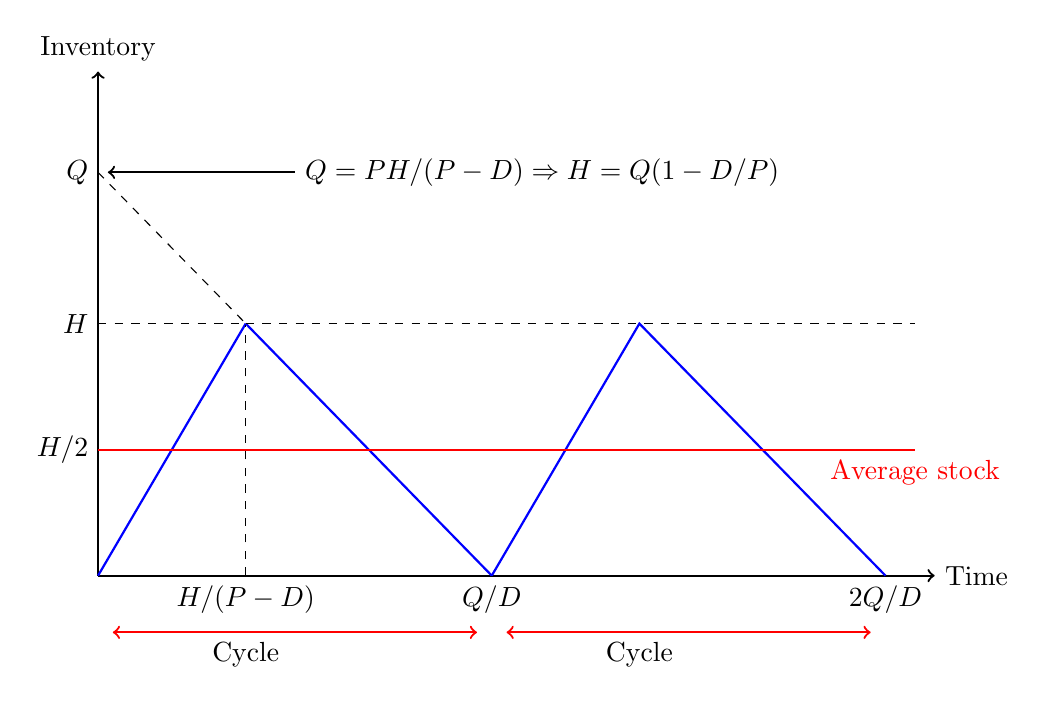
\begin{tikzpicture}[x=1.25cm,y=0.016cm]
\draw[thick,->] (0,0) -- (8.5,0) node[right] {Time};
\draw[thick,->] (0,0) -- (0,400) node[above] {Inventory};
\draw[] (0,200) node[left] {$H$};
\draw[dashed] (0,200) -- (1.5,200);
\draw[color=blue,thick] (0,0) -- (1.5,200);
\draw[] (1.5,0) node[below] {$H / (P-D)$};
\draw[dashed] (1.5,0) -- (1.5,200);
\draw[color=blue,thick] (1.5,200) -- (4,0);
\draw[dashed] (0,4*200/2.5) -- (1.5,200);
\draw[] (0,4*200/2.5) node[left] {$Q$};
\draw[] (4,0) node[below] {$Q / D$};
\draw[thick,<-] (0.1,4*200/2.5) -- (2,4*200/2.5) node[right] {$Q = PH / (P - D) \Rightarrow  H = Q(1 - D / P)$};
\draw[dashed] (1.5,200) -- (8.3,200);
\draw[color=blue,thick] (4,0) -- (4+1.5,200) -- (8,0);
\draw[] (8,0) node[below] {$2Q / D$};
\draw[] (0,100) node[left] {$H / 2$};
\draw[color=red,thick] (0,100) -- (8.3,100) node[below] {Average stock};
\foreach \y in {0,...,1}{
	\draw[color=red,thick,<->] (4*\y+0.15,-45) -- (4*\y+4-0.15,-45);
	\draw[] (4*\y+1.5,-45) node[below] {Cycle};}
\end{tikzpicture}
\caption{EPQ model}
\label{fig:EPQ}
\end{figure}

It is important to observe that the inventory behaves differently when production is on and off. If production is on, then the inventory increases with the rate $P-D$. Here $P$ stands for the production rate i.e. number of items produced in unit time. Note that $P$ is supposed to be larger than $D$, as it would otherwise be impossible to cover the demand. If production is off, the inventory process is the same with the classical model where it decreases with rate $D$. The production quantity in one cycle is $Q$. At the beginning of each cycle, production is switched on and it is switched off once $Q$ items have been produced. Because the inventories increase with rate $P-D$ during that time, we end up with $H=Q(1-\frac{D}{P})$ units once the machine has been turned off. Then production remains off until the inventory level drops down to zero, and then another cycle starts.

The total cost for one cycle is the sum of ordering cost, procurement cost, and inventory (holding) cost. The fixed setup cost (rather than fixed ordering) is $A$ per cycle as we switch on the machine only once in each cycle. The production cost (rather than procurement) equals the unit production cost times the order quantity $cQ$, i.e. we produce just enough to satisfy all the demand in each cycle. The inventory cost per cycle is the total area of the triangle times $h$, i.e. 
\begin{equation*}
h~\frac{\text{height}\cdot\text{base}}{2} = h~\frac{H \cdot Q/D }{2} = \left(1-\frac{D}{P}\right) \frac{h Q^2}{2D}.
\end{equation*}

Thus, the total cycle cost is $A+cQ+\frac{(1-\frac{D}{P}) h Q^2}{2D}$. The average cost per unit time is this total cost divided by the duration of one cycle, which is $\frac{Q}{D}$. Therefore, the average cost is
\begin{equation*}
A \frac{D}{Q}+cQ \frac{D}{Q} + \left(1-\frac{D}{P}\right) \frac{h Q^2}{2D} \frac{D}{Q} = \frac{AD}{Q}+cD+\left(1-\frac{D}{P}\right)\frac{hQ}{2}
\end{equation*}

This expression gives us the average cost as a function of the order quantity:
\begin{equation*}
f(Q) = \frac{AD}{Q}+cD+\left(1-\frac{D}{P}\right)\frac{hQ}{2}.
\end{equation*}

It is easy to observe at this point that we can derive the average cost function of the EPQ model simply by revising the holding cost $h$ of the EOQ model as $h'=h \left(1-\frac{D}{P}\right)$. All relevant results, such as expressions of the optimal order quantity and cost then immediately follows. For instance, the optimal production quantity $Q^*=\sqrt{\frac{2AD}{h'}}$ and optimal average cost per unit time $f(Q^*)=\sqrt{2ADh'}+cD$. The intuition behind is as follows. Let us assume that we are using the same $Q$ for the EOQ and EPQ models. Then the average stock level and thus the holding costs of the EPQ model will be $1-\frac{D}{P}$ times the average stock level of the EOQ model, and all other costs will be the same.  
\end{solution}
\end{exercise}

\begin{exercise}
For which parameter settings the optimal policies EOQ and EPQ models have a similar structure? 


\begin{solution}
Recall that the main difference between EOQ and EPQ models is that EOQ assumes the order arrive all at once and EPQ assumes items are produced with a fixed rate. Let us consider the EPQ model and assume that the production rate is extremely high. Then production becomes almost instantaneous. This setting should yield the same results with the EOQ model.

This is obvious if we look at the average cost function $f(Q) = \frac{AD}{Q}+cD+\frac{h'Q}{2}$ where $h'=h\left(1-\frac{D}{P}\right)$. If $P$ is very large, then 
$\left(1-\frac{D}{P}\right)$ approaches 1. Then $h'\approx h$ and we have the same cost function. For moderate values of $P$ the expression $\left(1-\frac{D}{P}\right)$ will be in between 0 and 1. Then $h'<h$ and it implies that the EPQ function is lower than the EOQ function.
\end{solution}
\end{exercise}

\begin{exercise}
How does the production rate affect the optimal production quantity and the average cost per unit time?


\begin{solution}
Let us consider the optimal production quantity $Q^*=\sqrt{\frac{2AD}{h'}}$ and corresponding optimal average cost per unit time $f(Q^*)=\sqrt{2ADh'}+cD$ where $h'=h\left(1-\frac{D}{P}\right)$. It is clear that the smaller the $P$ the smaller the adapted holding cost $h$. Then it is easy to see that a higher production rate leads to a smaller $Q^*$ and a higher $f(Q^*)$. 

We know that the production rate should be larger than the demand rate to be able to cover demand over time. Thus, the lowest feasible production rate is the demand rate itself. In this case we have $P=D$ and therefore $h'=h\left(1-\frac{D}{D}\right)=0$. The mathematics of this particular case is ill-defined to the division by 0. Nevertheless, it is easy to see what is going on. Because the production rate equals the demand rate; we simply have is no inventory! We switch on the machine and leave it switched on all the time. Thus we have neither fixed setup cost nor holding cost. All we need to pay is the production cost which is $cD$ per unit time.
\end{solution}
\end{exercise}

\begin{exercise}
It appears that having a slower production rate is favorable. How does this makes sense?

\begin{solution}
The issue is with the trade-off between setup and holding costs. If the machine is fast, then once you switch on you quickly build up inventories at a high speed. To avoid excessive inventories you switch off. But then you pay the setup cost more frequently. 
\end{solution}
\end{exercise}

\section{Capacitated production inventory system}
\label{sec:capac-prod-invent}



The basic inventory system we consider below consists of one machine with a certain (daily) production capacity to refill an inventory point downstream. Demand is served from this inventory point, if there is on-hand inventory, or otherwise backlogged or lost. We consider the inventory at the end of each day, hence, the model is a so-called \emph{discrete-time} model.

We use the following notation:
\begin{align*}
  d_i &= \text{demand arriving \emph{during} day $i$}, \\
  c_i &= \text{items produced (capacity) at the \emph{start} of day $i$}, \\
  I_i &= \text{Inventory on hand at the \emph{end} of day $i$}, \\
  B_i &= \text{Backlogged demand at the \emph{end} of day $i$}, \\
  S_i &= \text{Sales (number of demands met) \emph{during}  day $i$}, \\
\end{align*}
Mind the \emph{timing} of each variable.

\begin{exercise}
  Can you relate the production of the machine to a situation in which
  inventory is replenished by a supplier?

  \begin{solution}
    The production amount $c$ is equivalent to a constraint on the
    amount that can be ordered from a supplier. The time between
    deciding to produce and the moment an item is available for
    customers is equivalent to a lead-time between ordering a
    replenishment order and receiving the replenishment.
  \end{solution}
\end{exercise}


\subsubsection{Systems with backlogs but no inventories}

Generally, production situations without on-hand inventory are known as \emph{make-to-order (MTO)}.

\begin{exercise}\label{ex:2}
  Consider a production situation, a machine for instance, that has a
 maximal production capacity of $c$ per day, e.g. $c=10$.  The daily demand,
  $d_i$ for day $i$, is always less then $c$, and we assume the
  produced items on day $i$ are available at the start of the day. Is
  there a need for inventory?


  \begin{solution}
No. Since $c\geq d_i$, the daily demand can be covered by production every day again.     
  \end{solution}
\end{exercise}

\begin{exercise}
  Let's assume that the machine can be switched on or off.  If on, it
  produces at capacity $c_i=c$ jobs, if off it produces nothing.  Suppose there is no cost involved in switching on the machine, how would you control the   machine?
When is such cost structure reasonable?
  \begin{solution}
    We can just switch on the machine whenever there is a job. In
    fact, we can leave it on always, for there is no penalty to have
    it switched on (or a reward for switching it off).


    If you have to hire or assign personnel to operate the machine, you
    are typically confronted with a daily cost, whether the machine
    actually works or not.
  \end{solution}
\end{exercise}


\begin{exercise}
  Henceforth we assume that it costs $K$ Euro per day, for instance
  $K=100$ euro, just to have the machine switched on, whether you use
  the capacity or not. What would you do now? 
  \begin{solution}
    If $d_i=c$, i.e., the daily demand is always the same as the daily
    capacity, then there is not much you can do. However, if the
    demand is typically less than $c$, then it might be interesting to
    occasionally switch on the machine and let it produce all demand
    that accumulated up to some time. That is, ensure that the machine capacity $c$ can
    be completely used when it is switched on.  And when the machine is switched on, keep it on for a while.
  \end{solution}
\end{exercise}



\begin{exercise}\label{ex:3}
  Try to make a model for this case.  Use the checklist of Exercise~\ref{4step} to see what
  modeling choices you can (and have to) make.
  \begin{solution}
    Assume that customers are willing to wait for free.  Assume also
    that we want to serve all demand (note that this is a business
    decision as it might be profitable to reject some demand). Finally,
    assume that the demand process $\{d_i, i=1,2\ldots\}$ is given.

    You should realize at this point that capacity has a
    `lose-it-or-use-it' property. That is, unused capacity is lost and any
    (already paid) cost associated with that lost capacity is also lost.

    The best thing we can do then is to only switch on the machine
    when the total accumulated demand is larger than the capacity for
    a day.  Thus, if $d_1=2, d_2 = 5, d_3 = 4$, then take the capacity
    $c_1$ for day 1 equal to 0, and likewise for day 2. However,
    $c_3 =10$; recall the data from Exercise~\ref{ex:2}.

In more general terms,   take $c_i$ as the capacity of day $i$. In our case $c_i=c=10$ if
  production is on, and $c_i=0$ if production is off.  Realize that
  any unfilled demand is transferred to the next period. To keep track
  of total demand, let's call $B_i$ the total demand in the system
  waiting at the end of day $i$. % for the machine to make their item. 
Then, if the machine  does not produce anything in day $i$, the unfulfilled demand at the
  end of day $i$ is $B_i=B_{i-1}+d_i$, i.e., we start day $i$ with
  unfulfilled demand $B_{i-1}$ and the demand $d_i$ arriving on
  day $i$ adds to this. On the other hand, if the machine does produce, the total
  unfulfilled demand is
  \begin{equation*}
B_i = B_{i-1}-c_i + d_i =  B_{i-1} -10 + d_i.
  \end{equation*}
  since we produce $c_i=10$. Realize that this equation can easily be
  implemented in a spreadsheet.

Finally, observe that in the above we assume that when the machine is
on at day $i$, the  amount of demand served is  less than $B_{i-1}+d_i$, because otherwise
the $B_i<0$, and it is impossible to have a negative number of
customers in queue/backlog. To include this aspect,  the following formula can be used
    \begin{equation*}
    B_i = \max\{B_{i-1} + d_i - c_i, 0\}.
    \end{equation*}

    Fill in these formulas with a set of numbers for the demand and
    implement it in excel to see what happens.  Start doing all kinds
    of experiments. How sensitive is the result to changes in $c$, for
    instance? What is a good rule to switch on and off the machine?
  \end{solution}
\end{exercise}

Typically, the unfulfilled demand is called \emph{backlog}. The
interpretation is really simple, it is exactly the same as the queue
of customers waiting for capacity. If you would apply this reasoning
to the number of customers in queue waiting in a supermarket for
service you would obtain exactly the same result. Thus, once and for
all, backlogged customers, or backorders, are precisely the same thing
as a queue of jobs or customers waiting for capacity.

\begin{exercise}
  Implement the model of Exercise~\ref{ex:3} in a spreadsheet, and compute the total cost for the
  following demand process: $d = 2, 5, 4, 5, 0, 2, 3, 8, 9, 1, 1, 3$.
\begin{solution}
\nvf{to be done}
\end{solution}
\end{exercise}

\begin{exercise}
  Just in this exercise, we make a subtle change in our initial assumption on the capacity. 
  Let's assume that we can use the capacity on day $i$ just for the  
  demand that is in  backlog \emph{at the start of the day}. However, the capacity cannot serve demand $d_i$ that arrives \emph{during} day $i$.  How would you modify the model of Exercise~\ref{ex:3} to include this change?
  \begin{solution}
If the demand on day $i$ has to wait at least until day $i+1$, then
    \begin{equation*}
    B_i = \max\{B_{i-1} - c_i, 0\} + d_i.
    \end{equation*}

  \end{solution}
\end{exercise}
 


\begin{exercise}
  Can you find a set of formulas by which we can capture the relationship between the sales $S_i$, i.e., the amount of items sold on day $i$,  and the backlog at the end of day~$i$, assuming that the demand on day $i$ can be served by the producion on day $i$? 


  \begin{solution}
    Let's say that $S_i$ is the amount of demand sold on day $i$; in other words, $S_i$ is the amount of items that is fysically moved from the machine to the customers. In this case, the amount sold is 
    \begin{equation*}
      S_i = \min\{B_{i-1}+d_i, c_i\},
    \end{equation*}
    since we cannot produce/sell more than the demand in backlog and
    we can also not sell more than the capacity.  The backlog is therefore,
\begin{equation*}
  B_i = B_{i-1}+d_i - S_i.
\end{equation*}
  \end{solution}
\end{exercise}

\begin{exercise}
  Suppose that our decision to switch  the machine on and off would be independent
  of the amount of backlogged jobs. Can you find a formula, to be implemented in
  a spreadsheet, to compute the amount of capacity lost?
  \begin{solution}
The unused capacity $U_i$ is 
\begin{equation*}
  U_i = c_i - S_i,
\end{equation*}
because $c_i$ is the capacity we have, and $S_i$ is the amount we
used. Thus, all in all, 
\begin{align*}
      S_i &= \min\{B_{i-1}+d_i, c_i\}, \\
  U_i &= c_i - S_i, \\
  B_i &= B_{i-1}+d_i - S_i.
\end{align*}
Note that this scheme is quite simple in the sense that we have to
consider taking a minimum only once. It is very important to memorize this scheme.
  \end{solution}
\end{exercise}

For the rest of the course we need some important notation. 
\begin{exercise}
What is the meaning of $\sum_{i=1}^j x_i$ and why is $h \sum_{i=1}^j x_i = \sum_{i=1}^j (hx_i)?$
  \begin{solution}
    \begin{align*}
      \sum_{i=1}^3 x_i &= x_1 + x_2 + x_3 \\
      \sum_{i=1}^j x_i &= x_1 + x_2 + \cdots +x_j \\
     h \sum_{i=1}^j x_i &= h(x_1 + x_2 + \cdots +x_j) = hx_1 + \cdots+hx_j = \sum_{i=1}^j h x_i.
    \end{align*}
  \end{solution}
\end{exercise}

For the next exercise we introduce the so-called \emph{indicator
    function}, defined as
  \begin{equation*}
    \1{c_i>0} =
    \begin{cases}
      1, & \text{if } c_i > 0,\\
      0, & \text{if } c_i \leq 0.
    \end{cases}
  \end{equation*}
This function is also easy to implement in excel for instance. 


\begin{exercise}
Suppose it costs $p$ per day when  the machine is on. Explain that the total cost of operating the machine up to some day $n$ can be written as
    \begin{equation*}
      p \sum_{i=1}^j \1{c_i > 0},
    \end{equation*}
  \begin{solution}
Clearly,  we pay $p \1{c_i>0}$ for the production on day $i$. Thus, by adding up the costs for all periods we get the result.
  \end{solution}
\end{exercise}

\begin{exercise}
  Realize that in the previous problems we tacitly assumed that there
  is no cost associated with waiting.  In this case, we of course only
  switch on the machine when there is sufficient demand in
  backlog. But what would you do if it costs $b$ per day to keep one unit of demand
  waiting. Then it might not be so efficient, in terms of costs, to
  only switch on the machine when the demand is sufficiently high to
  prevent lost capacity. Can you find an expression for the total cost up to some day $j$ of
  keeping demand waiting?
  \begin{solution}
 On day $i$ we pay $b B_i$ if there are $B_i$ units of demand
    in backlog. Thus, the total backlogging cost up to time $j$ must be 
    \begin{equation*}
      b\sum_{i=1}^j B_i.
    \end{equation*}
  \end{solution}
\end{exercise}

\begin{exercise}
  Assume next that we get a profit $r$ per unit demand sold/produced, then
formulate the reward structure, including backlog and production cost.
  \begin{solution}
   The reward is the sum of the total profit minus the cost of backlog minus
    the cost of switching on the machine, thus,
    \begin{equation*}
     r \sum_{i=1}^j S_i - b \sum_{i=1}^j B_i - p \sum_{i=1}^j \1{c_i>0}.
    \end{equation*}
  \end{solution}
\end{exercise}


\begin{exercise}
  It might be that the business context requires that the amount of
  backlogged demand should not exceed some critical level $a$, say, too
  often. Can you find an expression to estimate, for instance with excel, how often such an
  event occurs? %  for a given set of demands?


  \begin{solution}
    When $B_i>a$ we are `in trouble'. Thus, to count how often this happen, we can compute
    \begin{equation*}
      \sum_{i=1}^j \1{B_i > a},
    \end{equation*}
as $\1{B_i>a}=1$ iff the backlog level exceeds level~$a$ at the end of day $i$.
  \end{solution}
\end{exercise}


\begin{exercise}
  Observe that in the previous exercise we only counted the number of
  periods (i.e., days) in which the backlogged demand exceeded some level $a$. It
  might also be of interest to compute the total amount of
 backlogged demand that exceeded the level $a$. What can be an appropriate formula for this? 
\begin{solution}
    When $B_i>a$, the amount in excess is $B_i-a$. Thus,  the total excess up to (the end of) day $j$ is
    \begin{equation*}
      \sum_{i=1}^j (B_i-a) \1{B_i > a}.
    \end{equation*}
\end{solution}
\end{exercise}


\begin{exercise}
As a check, can you relate the expression you found in the previous exercise to the total amount of demand backlogged? 
  \begin{solution}
    In the previous expression set $a=0$. 
  \end{solution}
\end{exercise}

%% lot sizing

\begin{comment}
  
\begin{exercise}[\faRocket]
 If you like, you can try to formulate an optimization problem for
 the problem on how much to produce. \tbd
 \begin{solution}

   TBD = to be done = unfinished. You can always skip exercises that
   are marked as TBD.

The decision variables are whether we switch on the machine at the days, i.e., $c_1, c_2, \ldots, c_j$. 

The constraints are:

\begin{align*}
c_i &\in \{0, 10\}, \\
     S_i &= \min\{B_{i-1}+d_i, c_i\}, \\
 B_i &= B_{i-1}+d_i - S_i.
\end{align*}

In Section 16.2 of Factory Physics it is shown how to optimize this
problem in excel for \emph{given} demand, i.e., if we know the
demands.  If we don't know the demands, then things become quite a bit
different.

\end{solution}
\end{exercise}

\end{comment}


\subsubsection{Systems with inventories}

\begin{exercise}
  In the previous section we assumed that customers are
  prepared to wait.  What if this is not the case, i.e., you serve
  them right away, or they are lost. Suppose we don't want demand to
  be lost. What can you do about this?


  \begin{solution}
 If we don't have inventories at the start of the day, all demand will be
    lost. Thus, the only way out is  keep real
    inventories. 

Realize that up to now we only considered backlogged
    demand, which is, in a sense, negative inventory.
  \end{solution}
\end{exercise}

\begin{exercise}
  Now, if we are willing to invest in on-hand  inventory, the question is of course:  How much inventory do we need? Supposing that  demand is capped by some number $\bar d$, i.e., all demands $d_i \leq \bar d$, how much inventory do we need?
  \begin{solution}
This depends entirely on the capacity of the machine. If we don't want to lose any demand, and we are always safe if we have $\bar d-c$ items on hand, i.e., on the shelf, at the start of a day, since if we produce $c$ on day $i$, it is right away available (by assumption) to serve the demand for day $i$. Thus, if $c\geq \bar d$, all is fine. 
  \end{solution}
\end{exercise}

\begin{exercise}
  If $c< \bar d$, the situation changes quite dramatically. Why, and what would you do about this?
  \begin{solution}
Suddenly,  to prevent loss we need more than $\bar d-c$ of inventory at the start
  of the day, because if the inventory becomes below $\bar d-c$, we
  might not be able to replenish it sufficiently for the next
  day. 

What would you do? First of all, we observe that it is impossible to prevent lost
    sales under all circumstances if demand is stochastic. It can
    happen that we have 10 days in row, say, that the maximal demand
    arrives. We need already quite a bit of inventory to cope with
    this. In general, in case demand is stochastic, any amount of
    demand can arrive, so that we cannot protect ourselves always
    against loss. Thus, we need \emph{safety stock} to compensate for the fact that
    our production cannot cope with the maximal daily demand. Tuning the safety stock to minimize cost is an issue we'll address
    next. 

    Typically, we assume that the capacity of the machine is higher
    than the average demand, for otherwise we will have quite a bit of
    loss. 
  \end{solution}
\end{exercise}

Based on the insights obtained from the previous exercices, we make a distinction now between inventory systems in which we allow for backlogging  and systems  with loss.

%\subsubsection{Systems with full backlogging}

\begin{exercise}
  Assume now that demand that cannot be covered by on-hand
  inventory will be  backlogged. Suppose further that  the machine operates under a \emph{basestock policy} with basestock level $r$: it produces an amount $c$ if the on-hand stock is below level $r$, and it is  off otherwise. Make a model of the behavior of the production-inventory system.
  \begin{solution}
    First of all, observe that we can absorb on-hand inventory and
    backlog into one concept. We write $I_i$ for the on-hand inventory
    at the end of the day if the on-hand inventory is positive and we
    set $I_i=-B_i$ if there is backlog. Thus, when $I_i$ is negative,
    it means that $I_i$ demand is in backlog.  Observe that, as a
    consequence, it cannot happen that there is demand in backlog but
    there is also positive on-hand inventory at the same time. With this notation, the expressions become particularly simple:
    \begin{align*}
      I_i &= I_{i-1}-d_i + c_i \\
c_i &= c \1{I_{i-1} \leq r}.
    \end{align*}
Observe, we do not take a minimum here.
  \end{solution}
\end{exercise}

% \begin{exercise}
%   Assume now that demand that cannot be covered by on-hand
%   inventory will be  backlogged. Make a model of the behavior of the production-inventory system when the machine works under a basestock policy, c.f., Exercise~\ref{ex:4}. 
%  and a cost function.
%   \begin{solution}
%     For the revenues we can also make at least two choices: do we get
%     the money when the customer decides to `enter the system',
%     irrespective of being backlogged, or do we get the money when we
%     actually satisfy the demand. Here we model the latter situation.
%     If $I_i\geq 0$, we know that we have met all demand for that
%     day. Thus, in this case, the sales for day $i$ must be
%     $S_i = d_i+B_{i-1}$, that is, the demand for day $i$ plus all
%     backlogged demand $B_{i-1}$, if any. If, however, $I_i <0$, then
%     we cannot have met $d_i$ entirely. Since we produced $c_i$ on that
%     day, $S_i = c_i$, i.e, we must have sold $S_i$. 

%     Note that we assume in the above that any items produced in excess
%     of $r$ is kept in inventory. If this is cannot be the case (due to
%     space restrictions for instance), the above recursions need to be
%     changed.

%     We leave it to you to consider other interesting cases and adapt
%     the above models to your settings.
%   \end{solution}

% \end{exercise}


% \begin{exercise}
%   nvf: 2018: below is a bit of nonsense, and also a sutble
%   question. I guess we don't want our students to learn this, so why
%   ask it?  How long does demand spend in backlog on average?
%   \begin{solution}
%     We can use Little's law to get an approximate value for this, but
%     it takes some time to see how to do it. So, let's review Little's
%     law. Consider some input-output system---it doesn't quite matter
%     what system, as long any item/job/customer that enter the system
%     eventually departs from the system.  Let jobs arrive at rate $r_a$
%     per unit time. The average time a job spends in the system is $W$
%     and the (time) average number of jobs in the system is $L$. Then
%     the law states that $L = r_a W$.  Thus, the average time jobs
%     spend in the system is $W = L/r_a$.

%     First consider the entire system. The rate at which jobs enter must be roughly 
%     \begin{equation*}
%       r_a = \frac 1 j \sum_{i=1}^j d_i,
%     \end{equation*}
%     i.e., the average demand rate. The time-average of the amount of
%     demand in backlog is roughly
%     \begin{equation*}
%     \bar B \approx \frac 1 j \sum_{i=1}^j B_i.
%     \end{equation*}
%     Hence, the average time demand spend in backlog must be
%     $W =  \bar B /r_a$.

%     Now notice that this is the average waiting time averaged over
%     \texttt{all} demand, thus, also the demand that actualy does not
%     have to wait. This number is therefore only partially interesting:
%     it doesn't tell how long, on average, a backlogged customer has to
%     wait. (Only when a customer has to wait, s/he is interested in how
%     long the waiting will take. Customers that don't have to wait, are
%     not interested in `knowing how long they have to wait'.) Thus, we
%     need to repair for this. But how? 

%     Well, we can again use Little's law, but now apply it to the
%     `system' that is entered only by the backlogged customers.  So,
%     how much demand enters this system?  A first guess is all the demand that leaves backlog behind:
%     \begin{equation*}
%       \sum_{i=1}^j d_i \1{B_i > 0}.
%     \end{equation*} 

%     Is this correct? What if $d_i=7$, $B_{i-1}=8$ and $c_i= 10$. Then
%     $B_{i} = 8+7-10 = 5$. Thus, assuming FIFO service of backlogged
%     demand, of the 7 demands entering, only 5 will be backlogged, the
%     rest, i.e., 2, will be served on day $i$ itself. That means that
%     $d_i \1{B_i>0}$ must overcount the amount of demand that is
%     backlogged. Another example might help to get the right number. If
%     $B_{i-1}=10$, the $B_i=7$, hence all demand on day $i$ is
%     backlogged. But if $B_{i-1}=2$, then $B_i = 0$ and no demand is
%     backlogged. Thus, only if $B_i\geq d_i$ all demand is backlogged,
%     otherwise $B_i$ is backlogged, in other words, 
%     \begin{equation*}
%       d_{i,b} = \min\{d_i, B_i\}
%     \end{equation*}
%     gets backlogged. The rate of  backlogged demand is then
%     \begin{equation*}
%       r_{a,b} =
%       \frac 1 n \sum_{i=1}^j d_{i,b} = \frac 1 n \sum_{i=1}^j \min\{d_i, B_i\}.
%     \end{equation*}
%     With this we see that the average time backlogged demand stays in
%     backlog must be
%     \begin{equation*}
%       W_b  = \frac{\bar B}{r_{a,b}}. 
%     \end{equation*}

%     Note that $r_{a,b} < r_a$, hence $W_b > W$, as it should.

%     It would be interesting to check the above with simulation, and
%     see whether any mistakes remain. 

%     Note also that we take the average over some $j$ periods. This is
%     of course not the same as the real long-run average (i.e., the
%     average taken over an infinite amount of time). As Little's law is
%     only valid asymptotically (taking an infinite amount of time), the
%     above relations can only be approximately correct.
%  \end{solution}

% \end{exercise}




% \subsubsection{Systems with loss}

% \begin{exercise}
%   Lets step back a bit\ldots In fact, we do not need to keep at least
%   $\bar d$ items of on hand inventory. What if we would carry less
%   inventory, and accept a bit of loss?  After all, the cost may
%   decrease if we allow for this situation. Can you make a model for
%   this situation, that is, a model that can cope with loss?


%   \begin{solution}
%     This is an interesting situation. First assume there is no
%     loss. Then the total amount we produce is the same as the total
%     demand. The production cost, i.e., cost to switch on the machine
%     is relatively simple. It is just the total demand divided by the
%     daily production capacity $c$ and then times the production cost
%     $p$ per day, in other words, the total cost of production up to period $j$ is
%     \begin{equation*}
%     \frac{p}c\sum_{i=1}^j d_i.
%     \end{equation*}

%     If there is loss, however, we need to produce less (because some
%     demand is lost) and we also can keep lower inventories. Thus,
%     accepting a bit of loss may be interesting as we get cost
%     reductions in two aspects: less production and lower inventories.
%   \end{solution}
% \end{exercise}

\begin{exercise}\label{ex:4}
Suppose that we would accept that demand, not covered by on-hand stock, is lost.  Can you find a set of equations to compute the on-hand inventory at day $i$, sales, and loss, based on the demand pattern, assuming that the machine works under a basestock policy?
  \begin{solution}
Observe that our sales $S_i$ in day $i$ may need not be equal to the demand $d_i$,  as we cannot sell more than what we have on stock. Thus,
    \begin{align*}
      c_i &= c \1{I_{i-1} \leq r}, &\text{ production} \\
      S_i &= \min\{d_i, I_{i-1}+c_i\}, &\text{sales }\\
      L_i &= d_i - S_i, & \text{loss}\\
      I_i &= I_{i-1} -S_i + c_i,  &\text{inventory}.
    \end{align*}
 Note that as $S_i \leq d_i$, $L_i \geq 0$, hence we don't run into a situation with of negative lost
    demand.
  \end{solution}
\end{exercise}


\begin{exercise}
  What would be the cost of this situation, assuming that it costs $k$
  per unit of demand lost, and $h$ per unit on-hand?
\begin{solution}
  \begin{equation*}
    \sum_{i=1}^j \left(h I_{i} + k L_i + p\1{c_i>0}\right).
  \end{equation*}
\end{solution}
\end{exercise}


\begin{exercise}
  How can you use the results of the previous two exercises to analyze  the production-inventory system? 
  \begin{solution}
. Observe that the control parameter is $r$, i.e., we can change the re-order level to influence the inventory level, sales and loss. By trying different choices for $r$ we
    can compute/simulate the inventory level, loss and so on, and the
    total cost. The best $r$ minimizes this cost.

    Realize that, formaly, it is not necessary that $c$ is larger than
    the mean demand. If it is less, simply more loss will occur.
  \end{solution}
\end{exercise}

\begin{exercise}
Find an expression to compute  the \emph{fill rate}, i.e., the fraction of demand met.
\begin{solution}
The total demand is
\begin{equation*}
 \sum_{i=1}^j d_i, 
\end{equation*}
and the total amount of demand served/sold is 
\begin{equation*}
 \sum_{i=1}^j S_i.
\end{equation*}
Hence, the fill rate is given by
\begin{equation*}
  \frac{\sum_{i=1}^j S_i}{\sum_{i=1}^j d_i}.
\end{equation*}
\end{solution}
\end{exercise}

\begin{exercise}
Find an expression to compute  the \emph{loss rate}, i.e., the fraction of demand lost.
\begin{solution}
\begin{equation*}
  \frac{\sum_{i=1}^j L_i}{\sum_{i=1}^j d_i} = 
  \frac{\sum_{i=1}^j (d_i-S_i)}{\sum_{i=1}^j d_i}.
\end{equation*}
\end{solution}
\end{exercise}

\begin{exercise}
Find an expression to compute  the \emph{service cycle level}, i.e., the fraction of periods in which loss did not occur:
\begin{solution}
Noting that $\1{L_i=0}=1$ if no loss occurs. Thus, the service cycle level is
\begin{equation*}
  \frac 1 j \sum_{i=1}^j \1{L_i=0}.
\end{equation*}
i.e., the average number of days in which the system did not run out of stock.
Note that fill rate and service cycle level are not the same. 
\end{solution}
\end{exercise}



\begin{exercise}
  Is the service cycle level a good measure for the  amount of loss?


  \begin{solution}
    No, not really. It might be that a small shortage occurs nearly
    every period. Then the fraction of periods without loss, i.e., the
    service cycle level, is very low. However, since only a small
    portion of the demand is lost, the fill rate may be pretty high. 

    So, why then use the service cycle level, and not always use
    fill rate? (Realize that fill rate does relate to money, but
    service cycle level doesn't.) Well, the answer is easy. People,
    managers in particular, tend to understand cycle service level
    better, and cycle service level is easy to compute. The fill rate
    is just a bit more complicated. 
  \end{solution}
\end{exercise}



\Closesolutionfile{ans}
\opt{solutionfiles}{
\subsection{Solutions}
\input{ans}
}

\clearpage

%%% Local Variables:
%%% mode: latex
%%% TeX-master: "inventory_notes"
%%% End:
